% $Header: https://svn.ita.chalmers.se/repos/security/edu/course/computer_security/trunk/assignment/3/template/latex/report.tex 611 2013-02-20 13:33:23Z pk@CHALMERS.SE $
%
%

\documentclass[a4paper,twoside,11pt]{article}

\usepackage{etoolbox}
\usepackage[utf8]{inputenc}
\usepackage{microtype}

\usepackage[pdftex,hidelinks]{hyperref}
\hypersetup{
    pdfstartview=FitH,
%    pdftitle={},
%    pdfauthor={},
%    pdfsubject={},
%    pdfkeywords={}
%    bookmarks,
%    bookmarksopen,
%    colorlinks,
%    linkcolor=blue,
%    citecolor=blue,
%    urlcolor=magenta,
}
\usepackage[english]{babel}
\usepackage[T1]{fontenc}
\usepackage{geometry}
\usepackage{fancyhdr}


% Setup bibliography
\usepackage{csquotes}
\usepackage[backend=biber, natbib=true, maxnames=2, minnames=1, 
maxbibnames=10, minbibnames=6, citestyle=numeric-comp, sorting=none, 
firstinits=true]{biblatex}
%\providecommand{\bibfont}{\footnotesize}
%\renewcommand{\bibfont}{\footnotesize}

% To be used for colors
\usepackage{color}
\usepackage[usenames,dvipsnames,svgnames,table]{xcolor}

% Useful Packages
\usepackage{amsmath}
\usepackage{amsthm}
\usepackage{amsfonts}

\usepackage{graphicx}
\usepackage{breakurl}

% Nice tables
\usepackage{hhline}
\usepackage{booktabs}
\usepackage{caption}

% Loading ToDo notes
\usepackage{setspace}
\usepackage{todonotes}
\usepackage{titlesec}
\newcommand{\inlinetodo}[2][]{\todo[caption={#2},inline,#1]{#2}}
\newcommand{\checknote}[2][]{\todo[caption={#2},size=\small,color=yellow!40,#1]{\begin{spacing}{0.5}#2\end{spacing}}}


\makeatletter
\renewcommand{\title}[1]{\gdef\@title{#1}}
\renewcommand{\author}[1]{\gdef\@author{#1}}
\renewcommand{\date}[1]{\gdef\@date{#1}}
\newcommand{\report}[1]{\gdef\@report{#1}}
\newcommand{\group}[1]{\gdef\@group{#1}}
\newcommand{\version}[1]{\gdef\@version{#1}}

\newcommand{\maketitlepage}{%
 \thispagestyle{empty}
 {
  \vspace{2cm}
  {\huge\centering\@title\par}
  \vspace{2cm}
  {\centering\@report\par}
  \vspace{2cm}
  {\centering\@author\par}
  \vskip1em
  {\centering\small Group~\@group\par}
  \vfill
  {\centering Version no:~\@version
   \vskip1em
   \@date\par}
  \vspace{2cm}

  \newpage
  \thispagestyle{empty}
  \mbox{}
 }
}
\makeatother

\renewcommand{\maketitle}{%
 \pagestyle{plain}
 \setcounter{page}{-100}
 \maketitlepage
 \newpage
 \pagenumbering{roman}
 \tableofcontents
 \cleardoublepage
 \pagenumbering{arabic}
}

% Title and Authors. This should be updated by you!
\title{Vulnerability Scanning with OpenVAS}
\report{Laboratory Report in EDA263/DAT641 Computer Security}
\author{Lluís Ripoll\\ Olle Svensson}
\group{45}
\date{\today}
\version{1.0}

% The bilbiography to include
\addbibresource{report.bib}


\begin{document}

\maketitle % Make titlepage

\newcommand{\sectionbreak}{\clearpage}

\section{Introduction} \label{sec:intro}

In this assignment we used the OpenVAS vulnerability scanning tool to gather information about and to assess the security of a system (remote computer) used for the identification and correction of security flaws. Vulnerability Assessment is a technique used to evaluate resources and assets present in a company. This type of audit is based on the identification of open ports, available services and from this the detection of possible failures present in the target systems. The purpose is to know what vulnerabilities exist in a company's systems and thereby develop an appropriate action plan.
In this way, a security assessment can be carried out on the systems of an organisation in order to increase security in them. In addition to this activity, there are other concerns, so it is necessary to complement it with security solutions, such as those against malicious code, firewalls, intrusion detection tools and good security policies contribute to the protection of asset and the combination of different approaches to security. 
First of all we had to get familiar with how OpenVas works (interface as well) and try to understand the framework and it's different options and parameters. Then it comes the analysis part, because is really important to understand the different vulnerabilities that a system can has as well as find a way to solve them making the system more secure.  
\newline


\section{Description of OpenVAS Setup} \label{sec:setup}

OpenVAS Is a framework that offers services and tools that provide a complete and powerful solution for vulnerability scanning and vulnerability management as well as it allow us to identify different security risks in a system (not only scan ports). So the main aim of OpenVAS is to assert a system (vulnerability identification). At the same time it allows us to make several types of reports on detected vulnerabilities and to propose associated solutions. In relation with the architecture, OpenVAS consists in the client part (OpenVAS CLI command line/Greenbone assistant) that interacts with two services called OpenVAS scanner (core) and OpenVAS management (back-end part). The first one performs tasks related with classification/filtering of the scanned results, database control and user administration. On the other hand the OpenVAS scanner executes the NVT (Network Vulnerability Test) conformed by routines that check known vulnerabilities into the system.

In figure 1, the network setup is described as clients connecting to the OpenVAS server ($theoden.ce.chalmers.se$ and in our case in a remote way SSH) via the client Greenbone that manages the  requests and send them to the OpenVAS Manager in order to scan the hosts. In this case the network contains 3 hosts (this report is based on scans of $rome.secnet$).

Scanning methods allow to detection and handling of known security problems, can help identify rogue machines on the network and provide useful information about the 	devices that can be useful in security management and tracking.
There are different types of vulnerability scanning such as network-based that scans a 	number of hosts on the network (port scanners, web application scanners) and host-	based scanners where the same host is scanned.

The scanning results tell us the results of the prioritised vulnerabilities (high, 	medium, low) according to the impact on the system and the total amount for each category. In our case we made a scan against the target host $rome.secnet$ and no 	vulnerabilities have been found. Once the scan has finished one vulnerability 	assessment report is available giving us useful information. It contains the results of the executed plugins associated with the corresponding subnet, host, port and severity.

To perform as scan using OpenVAS, a new target has to be created by clicking on Configuration/add a new 	target. Once there, some fields have to be filled (Name, host IP, port list). After, is it necessary to generate a new task clicking on scan management/new task for the execution of the analysis and evaluation. Finally the task must be executed and a report with the results is generated.

%\inlinetodo{Why you choose the different NVTs and the chosen configurations?}

Depending on your needs and your budget there are a number of different well known vulnerability scanners available. Furthermore, multiple options are available depending on the type of system to be tested. For example scanning all ports in many cases takes too long. Many ports are normally not being used. For most scans it is often enough to scan the ports registered with the IANA.

\begin{figure}[htb]
  \centering
  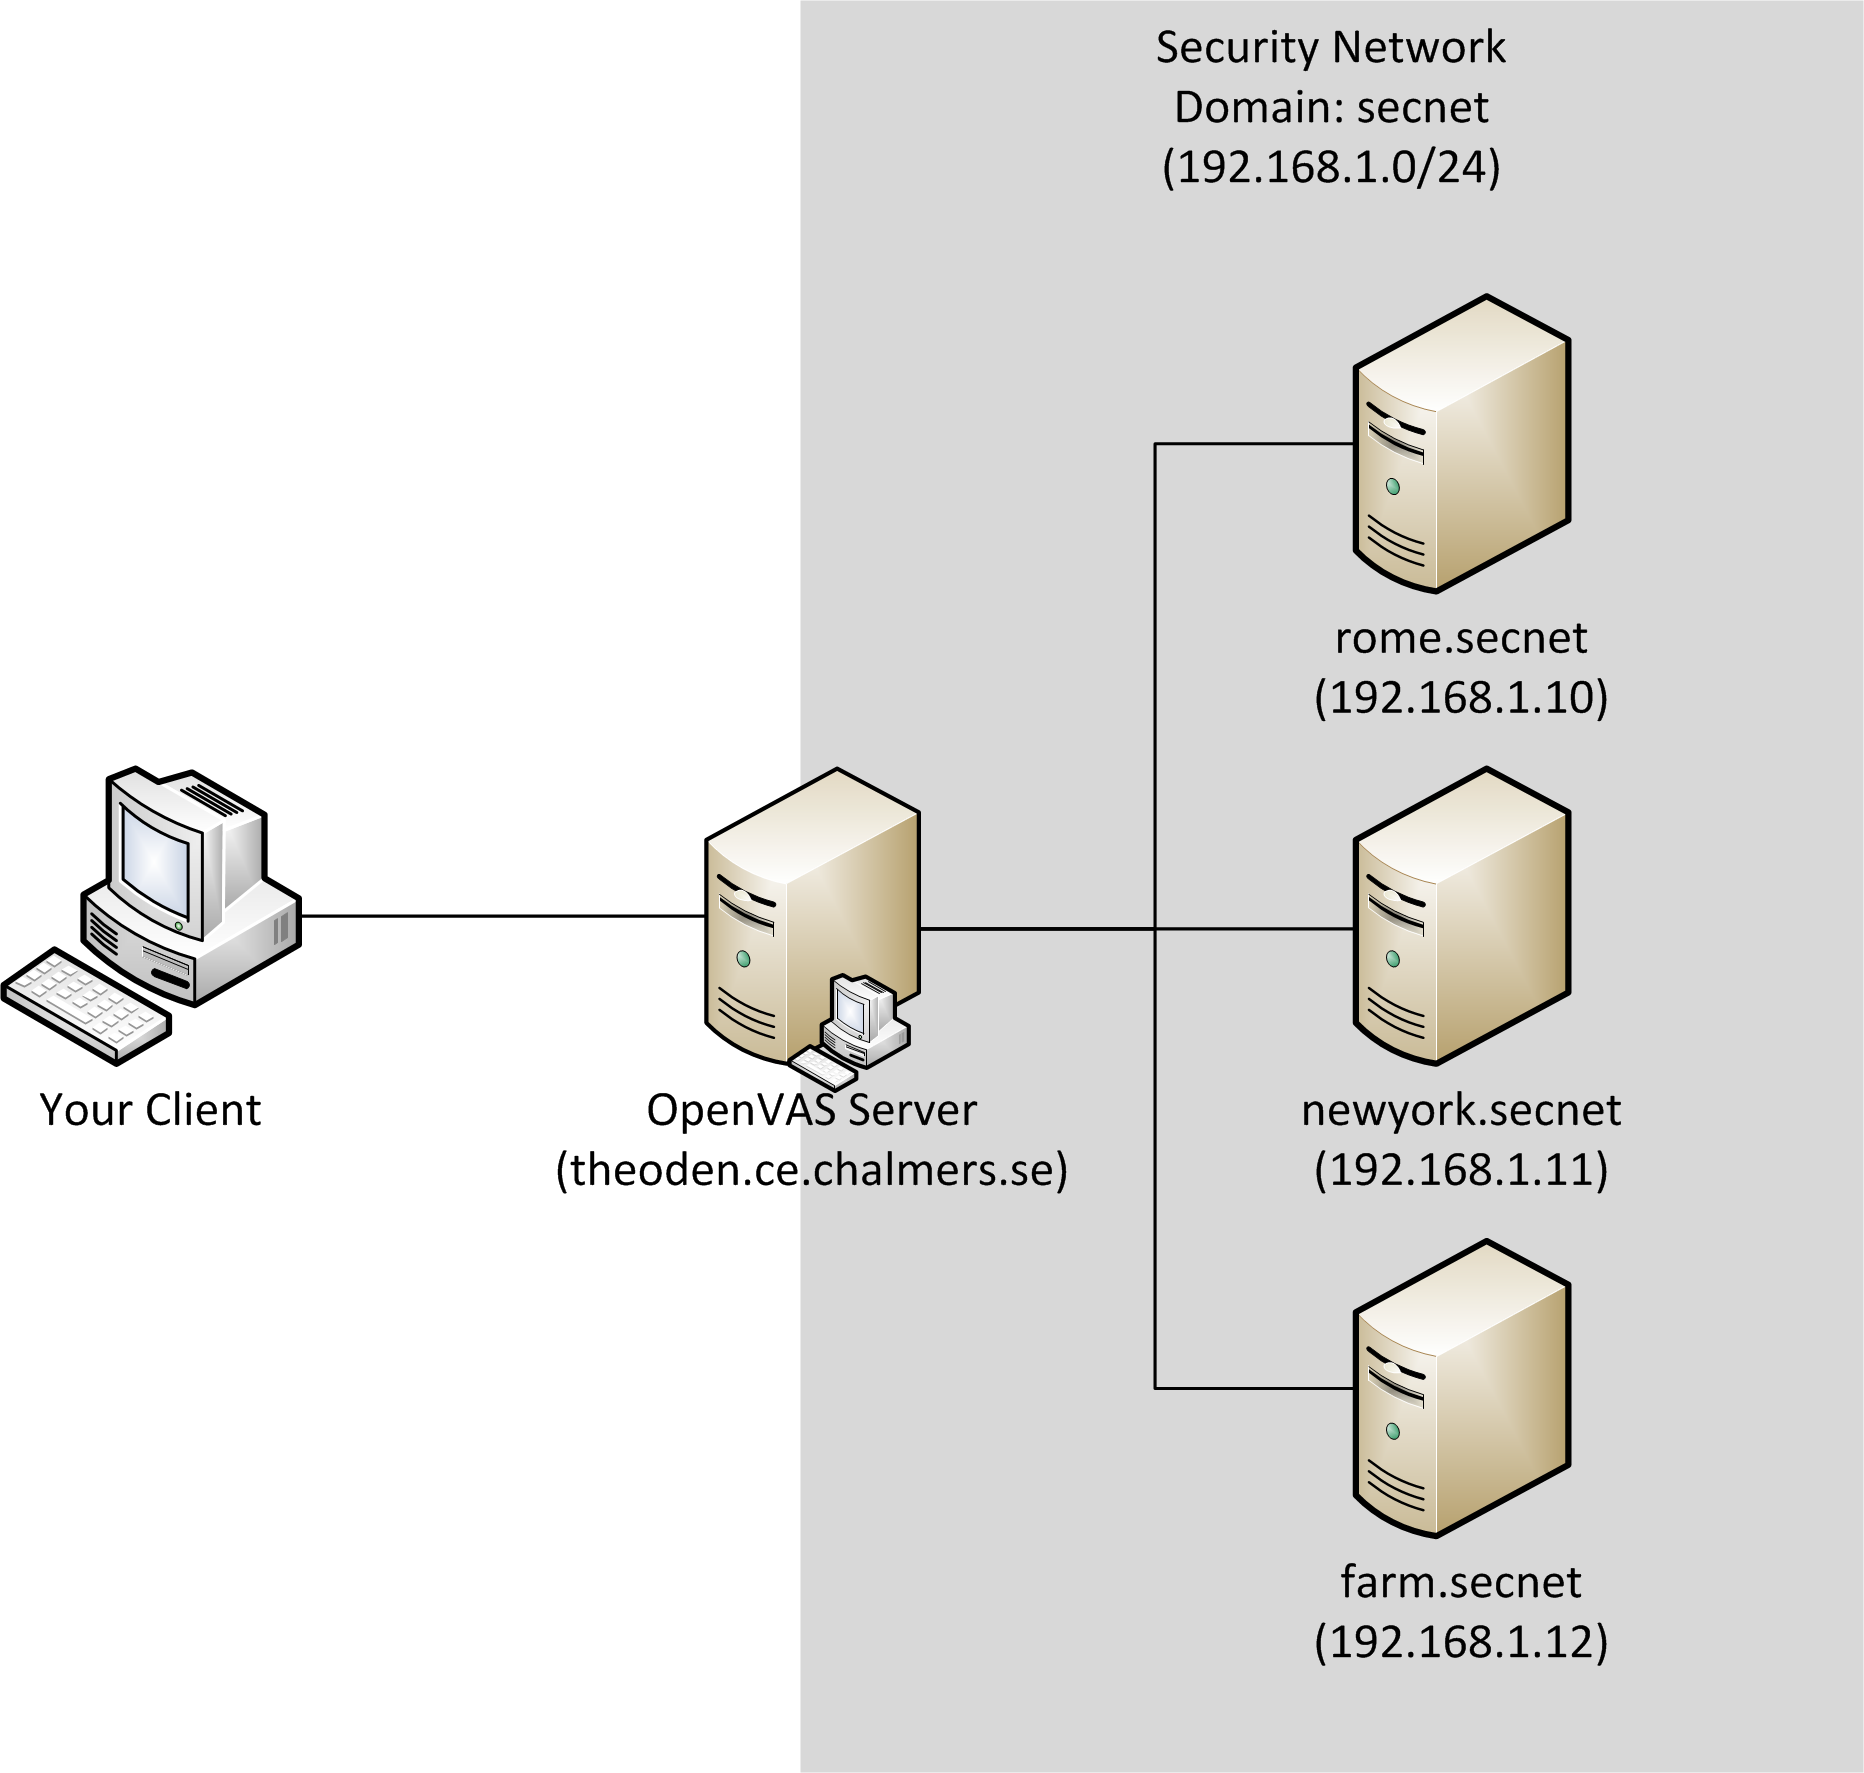
\includegraphics[scale=.4]{figures/setup.png}
  \caption{The laboratory network setup} \label{fig:setup}
\end{figure}



%\subsection{Port Scanning}

%\inlinetodo{text, figures, and tables if needed. Figure captions are below of figures, and Table caption should be above them.}


%\subsection{Fingerprinting}

%\inlinetodo{text, figures, and tables if needed}


%\subsubsection{Service Fingerprinting}
%\inlinetodo{text, figures, and tables if needed}

%\subsubsection{Remote Host Fingerprinting}
%\inlinetodo{text, figures, and tables if needed}


%\subsection{Vulnerability Scanning}

%\inlinetodo{text, figures, and tables if needed}

\section{Results}

\subsection{Port Scanning}

A port is a logical construct that identifies a specific process or a type of network service. The port scan that we performed used the scan config port scanners. The ports mentioned in the report (open ports on the remote system) are known as well-known because they are used by system processes that provide widely used types of network services. Is really important to test all ports in order to achieve security verification and the  main reason is that networks ports are the entry points to a machine that is connected to the Internet. A service that listens on a port is able to receive data from a client application, process it and send it back and consequently, malicious clients can take advantage of it.

The scan found 10 open TCP ports in total from the OpenVAS default range of ports. The open ports are used for standard services like mail, web browsing and file and printer sharing. No significant threats, a few minor issues regarding the services \textit{domain}, \textit{microsoft-ds} and \textit{ssh} that could be evaluated further if needed.


\begin{table}[htb]
 \centering
 \caption{Information about open ports} \label{tab:open_ports}
 \begin{tabular}{m{1.8cm}m{1.5cm}p{5.7cm}p{3.7cm}} \toprule
 \textbf{Port Number} & \textbf{Service Name} & 
 \textbf{Service Task} & 
 \textbf{Suggestions} \\ \midrule
 53 	& domain		& Used for DNS services. & Could expose a list of all computers connected to the internal network through a \textit{zone transfer} request. If this is considered sensitive information, incoming TCP requests on this port should be blocked.\\
 80 	& http			& Used for sending and receiving HTTP-requests. & Should remain open if the network is to support the usage of web browsers.\\
 8080 	& http-alt		& Alternative port for offering web services through HTTP. & Mostly used for hosting web services when port 80 is unavailable. The port could be closed if it is not used for this purpose. \\
 143	& imap			& Used to retrieve mail from remote mail servers. & Should be kept open if the network wishes to support mail clients.\\
 993	& imaps			& IMAP over SSL. & Should be kept open if the network wishes to support mail clients.\\
 445	& mircosoft-ds	& Used for Windows file sharing and numerous other services. & Used by the SMB protocol which has had multiple vulnerabilities in the past. Should be closed if not needed. If needed, make sure that the services using it support secure authentication protocols. \\
 139	& netbios-ssn	& A protocol used for file and print sharing under all current versions of Windows. & Should remain open if the network wants to support file and print sharing. \\
 110	& pop3			& Used by mail clients for retrieval of mail from designated mail servers. & Keep open to support mail clients or servers. \\
 995	& pop3s			& POP3 over SSL. & Keep open to support mail clients or servers. \\ 
 22		& ssh			& Used for the SSH remote login protocol. & SSH has contained vulnerabilities in the past. Close if SSH access is not needed. \\ \bottomrule
 \end{tabular} 
\end{table}


\subsection{Fingerprinting}


\subsubsection{Services}

The scan was unable to retrieve any version information from the targeted services even when extending the range of ports and selecting all available NVT's in the categories General and Service Detection.

The only service information retrieved was from the DNS server which is an open-source variant called BIND 'NAMED' running on version 9.7.0-P1.

\begin{table}[htb]
 \centering
 \caption{Service fingerprint} \label{tab:service_fingerprint}
 \begin{tabular}{m{2cm}p{5cm}} \toprule
 \textbf{Service} & \textbf{Version} \\ \midrule
 Telnet & \textit{unknown} \\
 FTP & \textit{unknown} \\
 SSH & \textit{unknown} \\
 SMTP & \textit{unknown} \\
 WWW & \textit{unknown} \\ \bottomrule
 \end{tabular} 
\end{table}


\subsubsection{Remote Host}

As with services, the scan was unable to retrieve any information regarding the host operating system or architecture.


\subsection{Vulnerability Scan}

The scan found a total of 7 high threats and 14 medium threats. All high threats are related to outdated versions of Apache and OpenSSL applications. The majority of the medium threats are related to outdated versions as well. Remaining errors consists of two configuration issues and a expired certificate.
\section{Discussion} \label{sec:discussion}

The scanning of ports did not reveal anything out of the order. However the applications using the open ports and services contain multiple security issues. As mentioned in Table 1, if these services are not needed, they should be closed to avoid the issues altogether. If the applications and services are to remain, the common solution for the majority of them is to update the software to the latest version. Since multiple vulnerabilities were considered as high risk, whatever decision the company decides to make should be done as soon as possible. 
\begin{table}[htb]
 \centering
 \caption{Summary of vulnerability scan recommendations} 
 \label{tab:recommendations}
 \begin{tabular}{m{2cm}p{4cm}p{7cm}} \toprule
 \textbf{Service Name} & \textbf{Problems} & \textbf{Suggestions} \\ \midrule
 http, http-alt 	& Outdated versions of Apache, Apache HTTP Server and Apache Tomcat. Enables multiple security vulnerabilities. Existing example files could expose version information. & Update to latest version and remove example files. \\
 imap, imaps, pop3, pop3s & Outdated version of OpenSSL. Enables man in the middle security bypass. & Updated to latest version. \\
 tcp & TCP timestamps could possibly expose system uptime. & Disable TCP timestamps. \\
 netbio-ssn & Outaded version of Samba which enables denial-of-service vulnerabilities. & Update to latest version. \\
 imaps, pop3s & The SSL certificate has expired. & Renew the certificate. \\ 
 ssh & Outdated version. & Update to latest version. \\ \bottomrule
 \end{tabular} 
\end{table}


\section{Conclusion} \label{sec:conclusion}

Even though the current system contains multiple security threats, these could be easily fixed and avoided by applying a basic security policy.
Most importantly, the company should introduce regular checks to ensure that the software running on their server is up to date.
Second, they should introduce a regular task to renew their SSL certificate to make sure that it does not expire.
If possible, the company should perform regular vulnerability checks as well to find any new threats that might be introduced when making new configurations on the server.

By applying this simple policy, the company should retain decent protection against common vulnerabilities and attacks.


%\printbibliography


\appendix
\cleardoublepage
%\section{Report from OpenVAS Vulnerability Scanning}

\inlinetodo{Possibly include your report from your full scan with OpenVAS.}

\end{document}

